% Options for packages loaded elsewhere
\PassOptionsToPackage{unicode}{hyperref}
\PassOptionsToPackage{hyphens}{url}
%
\documentclass[
]{article}
\usepackage{lmodern}
\usepackage{amssymb,amsmath}
\usepackage{ifxetex,ifluatex}
\ifnum 0\ifxetex 1\fi\ifluatex 1\fi=0 % if pdftex
  \usepackage[T1]{fontenc}
  \usepackage[utf8]{inputenc}
  \usepackage{textcomp} % provide euro and other symbols
\else % if luatex or xetex
  \usepackage{unicode-math}
  \defaultfontfeatures{Scale=MatchLowercase}
  \defaultfontfeatures[\rmfamily]{Ligatures=TeX,Scale=1}
\fi
% Use upquote if available, for straight quotes in verbatim environments
\IfFileExists{upquote.sty}{\usepackage{upquote}}{}
\IfFileExists{microtype.sty}{% use microtype if available
  \usepackage[]{microtype}
  \UseMicrotypeSet[protrusion]{basicmath} % disable protrusion for tt fonts
}{}
\makeatletter
\@ifundefined{KOMAClassName}{% if non-KOMA class
  \IfFileExists{parskip.sty}{%
    \usepackage{parskip}
  }{% else
    \setlength{\parindent}{0pt}
    \setlength{\parskip}{6pt plus 2pt minus 1pt}}
}{% if KOMA class
  \KOMAoptions{parskip=half}}
\makeatother
\usepackage{xcolor}
\IfFileExists{xurl.sty}{\usepackage{xurl}}{} % add URL line breaks if available
\IfFileExists{bookmark.sty}{\usepackage{bookmark}}{\usepackage{hyperref}}
\hypersetup{
  hidelinks,
  pdfcreator={LaTeX via pandoc}}
\urlstyle{same} % disable monospaced font for URLs
\usepackage[margin=1in]{geometry}
\usepackage{graphicx,grffile}
\makeatletter
\def\maxwidth{\ifdim\Gin@nat@width>\linewidth\linewidth\else\Gin@nat@width\fi}
\def\maxheight{\ifdim\Gin@nat@height>\textheight\textheight\else\Gin@nat@height\fi}
\makeatother
% Scale images if necessary, so that they will not overflow the page
% margins by default, and it is still possible to overwrite the defaults
% using explicit options in \includegraphics[width, height, ...]{}
\setkeys{Gin}{width=\maxwidth,height=\maxheight,keepaspectratio}
% Set default figure placement to htbp
\makeatletter
\def\fps@figure{htbp}
\makeatother
\setlength{\emergencystretch}{3em} % prevent overfull lines
\providecommand{\tightlist}{%
  \setlength{\itemsep}{0pt}\setlength{\parskip}{0pt}}
\setcounter{secnumdepth}{-\maxdimen} % remove section numbering

\author{}
\date{\vspace{-2.5em}7/1/2020}

\begin{document}

{
\setcounter{tocdepth}{2}
\tableofcontents
}
\hypertarget{updating-your-v1-sensorstation-radios-to-detect-new-hardware}{%
\section{Updating your V1 SensorStation Radios to Detect New
Hardware}\label{updating-your-v1-sensorstation-radios-to-detect-new-hardware}}

\hypertarget{why-update}{%
\subsection{Why Update?}\label{why-update}}

This is a valid question. In 2020 we introduced the 2nd version of the
\texttt{CTT\ SensorStation}, and simultaneously released new versions of
the \texttt{CTT\ Node} and \texttt{CTT\ LifeTag}. For the latter two
products we made some significant advances in the way they communicate
with our SensorStation radios, and they way they confirm their digital
ID. Technology moves at lightning speed, and while we made these changes
with every intention of full backwards compatibility, we soon learned
that the radios would need to be manually updated once before they could
join the V2 SensorStations in receiving over-the-air radio programming.

\emph{So should you update?} If you plan to add
\texttt{Version\ 2\ CTT\ Nodes} to your study, then the answer is
absolutely \textbf{yes}. If your station is
\texttt{listening\ for\ V2\ LifeTags}, it will still pick up the tag ID
like it always has, but will not be able to use the tag ID confirmation
code to absolutely validate the ID. So if you want the highest degree of
confirmation for LifeTags, then the answer is also \textbf{yes}.

If you're doing a localized study using PowerTags and not using any of
the newer Nodes, then you don't need to update the radios at
all\ldots{}\emph{but of course you still can!} To find out how, read
on\ldots{}

\hypertarget{getting-started}{%
\subsection{Getting Started}\label{getting-started}}

\hypertarget{things-youll-need}{%
\subsubsection{Things you'll need}\label{things-youll-need}}

\begin{itemize}
\tightlist
\item
  \textbf{USB Programmer with a ribbon cable} and 6-pin female header
  (if male header exists on your V1 station radios) or male header (if
  no header exists on your V1 station radios)

  \begin{itemize}
  \tightlist
  \item
    If your V1 SensorStation radios do not have headers, you'll also
    need this part to make the connection between the programmer cable
    and the board: \href{https://www.sparkfun.com/products/12807}{click
    here}
  \item
    We recommend this programmer:
    \href{https://www.amazon.com/USBtinyISP-Programmer-Bootloader-Download-Interface/dp/B01FDD4EP0/ref=sr_1_1?crid=3AEXHPTVD9KER\&dchild=1\&keywords=usbtinyisp\&qid=1593638163\&sprefix=usbtiny\%2Caps\%2C149\&sr=8-1}{click
    this here}
  \item
    but this one will also work with a little more effort (PC-only):
    \href{https://www.amazon.com/ARCELI-USBASP-USBasp_H6-Programmer-Support/dp/B0785RQ766/ref=sr_1_12?dchild=1\&keywords=bootloader\&qid=1593638232\&s=electronics\&sr=1-12}{click
    here}

    \begin{itemize}
    \tightlist
    \item
      \textbf{If you are using this programmer, or having issues with
      your \texttt{USBtinyISP} see
      \protect\hyperlink{troubleshooting}{Troubleshooting} for special
      instructions before proceeding.}
    \end{itemize}
  \end{itemize}
\item
  \textbf{Computer} (Mac or PC)
\end{itemize}

\hypertarget{part-1-setting-up-arduino-ide}{%
\subsection{Part 1: Setting up Arduino
IDE}\label{part-1-setting-up-arduino-ide}}

\begin{enumerate}
\def\labelenumi{\arabic{enumi}.}
\tightlist
\item
  Using your favorite browser, navigate to \url{http://arduino.cc}
\item
  From the main page, select \texttt{Software} \textgreater{}
  \texttt{Downloads}
\item
  Download the Arduino IDE *
\end{enumerate}

\begin{itemize}
\tightlist
\item
  (* if using the USBasp device, you must download
  \texttt{Arduino\ IDE\ 1.6.9} or earlier. You can do so
  \href{https://www.arduino.cc/en/main/OldSoftwareReleases}{here}).
  Again, see \protect\hyperlink{Appendix_I}{Appendix I} for full
  instructions for using that programmer.
\end{itemize}

\begin{enumerate}
\def\labelenumi{\arabic{enumi}.}
\setcounter{enumi}{4}
\tightlist
\item
  From the \texttt{File} menu, select \texttt{Preferences}
\item
  Near the bottom of the \texttt{Preferences} page you'll see a window
  for \texttt{Additional\ Boards\ Manager\ URLs}. Past the following in
  that window:
\end{enumerate}

\begin{verbatim}
https://adafruit.github.io/arduino-board-index/package_adafruit_index.json
\end{verbatim}

\begin{enumerate}
\def\labelenumi{\arabic{enumi}.}
\setcounter{enumi}{4}
\item
  Now go to \texttt{Tools} \textgreater{} \texttt{Board\ “xxx”}
  \textgreater{} \texttt{Boards\ Manager}
\item
  Install the latest version of \texttt{Adafruit\ AVR\ Boards}
\item
  Now the Adafruit boards will appear un the \texttt{Tools}
  \textgreater{} \texttt{Board:”xxx”} menu\ldots choose
  \texttt{Adafruit\ Feather\ 32u4}
\end{enumerate}

\emph{At this point you are almost ready to connect the adapter on the
USBtinyISP to the header on the SensorStation radios and burn the new
bootloader on each radio, but first we have a little prep work to
do\ldots{}}

\begin{enumerate}
\def\labelenumi{\arabic{enumi}.}
\setcounter{enumi}{5}
\item
  Connect the USBtinyISP device to your compute using a USB cable.
\item
  Go to \texttt{Tools} \textgreater{} \texttt{Programmer} and select
  \texttt{USBtinyISP}
\end{enumerate}

\hypertarget{part-2-prepping-your-sensorstation-for-updating-the-radios}{%
\subsection{Part 2: Prepping your SensorStation for updating the
radios}\label{part-2-prepping-your-sensorstation-for-updating-the-radios}}

\begin{enumerate}
\def\labelenumi{\arabic{enumi}.}
\tightlist
\item
  Ensure the SensorStation is \texttt{OFF}, and the \textbf{power has
  been disconnected}.
\item
  Remove the Raspberry Pi module by carefully pushing apart the tabs
  holding the Pi in place. This will cause the Pi to pop out at an angle
  from the top of the Pi (the bottom is hinged), at which point you can
  remove it by pulling up at an angle.
\end{enumerate}

\begin{figure}
\hypertarget{id}{%
\centering
\includegraphics[width=0.25\textwidth,height=\textheight]{/Users/davidlapuma/github/ctt_documentation/images/removePiOpt.GIF}
\caption{removing the Raspberry Pi Module}\label{id}
}
\end{figure}

\begin{enumerate}
\def\labelenumi{\arabic{enumi}.}
\setcounter{enumi}{2}
\tightlist
\item
  Set the Raspberry Pi aside.
\end{enumerate}

\hypertarget{part-3-burning-the-bootloader-on-the-radios}{%
\subsection{Part 3: Burning the Bootloader on the
Radios}\label{part-3-burning-the-bootloader-on-the-radios}}

\textbf{The first step of Part 3 will differ depending on whether your
V1 SensorStation came with the radio programming headers or not (whether
there are six holes, or six pins, in a 2x3 grid just above the radio SMA
ports). The directions below are written assuming no headers are
present, so the header pins are on the end of the adapter instead. If
your board has headers already, simply insert the female 6-pin header
onto the radio pins instead.}

\begin{enumerate}
\def\labelenumi{\arabic{enumi}.}
\item
  Place the adapter pins into the holes on the header for the first
  radio (\textbf{Note: You will need to apply some downward pressure to
  ensure a connection to the header.})

  \begin{figure}
  \hypertarget{id}{%
  \centering
  \includegraphics[width=0.25\textwidth,height=\textheight]{/Users/davidlapuma/github/ctt_documentation/images/attachProgrammerOpt.GIF}
  \caption{Connecting the programmer to the radio programming
  header}\label{id}
  }
  \end{figure}
\item
  With the adapter connected to the header, from the \texttt{Tools} menu
  on the Arduino IDE click \texttt{Burn\ Bootloader}.
\item
  At this point you will see dialogue on the Arduino IDE interface
  indicating that the Bootloader is being burned on to the radio. This
  should take less than a minute for each radio. Once it is complete,
  the radio light will be pulsing red.
\item
  Repeat steps 3.1 - 3.3 for each of the remaining four 434MHz radios
\end{enumerate}

\textbf{You're done!\ldots well, almost\ldots{}}

\hypertarget{part-4-running-the-radio-update-software}{%
\subsection{Part 4: Running the Radio Update
Software}\label{part-4-running-the-radio-update-software}}

Now that the radios are reprogrammed, you will need to SSH into your
SensorStation, so\ldots{}

\begin{enumerate}
\def\labelenumi{\arabic{enumi}.}
\item
  reconnect the power and connect to your station via the Ethernet
  adapter, or by plugging it into a router and accessing the IP over
  your local internet.
\item
  Download the following three files to your Downloads folder:
\end{enumerate}

\texttt{ssr\_v2\_3\_1.ino.hex} \texttt{program-radio.sh}
\texttt{program-radios\_sh.sh}

\begin{enumerate}
\def\labelenumi{\arabic{enumi}.}
\setcounter{enumi}{2}
\item
  Open the PowerShell Command Prompt (PC) or Terminal (Mac)
\item
  Change your directory to the Downloads folder:
\end{enumerate}

On Mac: \texttt{cd\ \textasciitilde{}/Downloads}

On PC: \texttt{cd\ Downloads}

\begin{enumerate}
\def\labelenumi{\arabic{enumi}.}
\setcounter{enumi}{4}
\tightlist
\item
  Run the following lines of code, replacing the words
  \texttt{sensorstation.local} with the \textbf{IP address} of your
  SensorStation. So, for instance, if your station IP address is
  \texttt{255.255.233.0} the first \texttt{scp} command above would read
  \texttt{scp\ ssr\_v2\_3\_1.ino.hex\ pi@255.255.233.0:/home/pi/}.
\end{enumerate}

\begin{verbatim}
scp ssr_v2_3_1.ino.hex pi@sensorstation.local:/home/pi/
scp program-radio.sh pi@sensorstation.local:/home/pi/
scp program-radios_sh.sh pi@sensorstation.local:/home/pi/program-radios.sh
ssh pi@raspberrypi.local 
sudo su
mv ./program-radio.sh /usr/sbin/program-radio
chmod a+x /usr/sbin/program-radio
chmod a+x ./program-radios.sh
./program-radios.sh ./ssr_v2_3_1.ino.hex
\end{verbatim}

\textbf{You should now see your radio lights now switch off, and only
blink when detecting tags.}

\hypertarget{step-5-flashing-a-compute-module-for-a-sensorstation}{%
\subsection{Step 5: Flashing a Compute Module for a
SensorStation}\label{step-5-flashing-a-compute-module-for-a-sensorstation}}

Now that you've updated the radios, you'll need to update your
SensorStation to detect the newer tags and nodes.

You can use the Sensor Station to burn a new operating system onto the
compute module using a micro USB cable attached to your computer.

Please follow the directions here to do so:
\url{https://woodcreeper.github.io/ctt_documentation/flashingComputeModule.html}

\hypertarget{troubleshooting}{%
\subsection{Troubleshooting}\label{troubleshooting}}

Programmer drama! So it appears all programmers are not created equal.

\hypertarget{im-having-issues-with-usbtinyisp}{%
\subsubsection{\texorpdfstring{I'm having issues with
\texttt{USBtinyISP}}{I'm having issues with USBtinyISP}}\label{im-having-issues-with-usbtinyisp}}

Try this\ldots{}

\begin{enumerate}
\def\labelenumi{\arabic{enumi}.}
\tightlist
\item
  Go to
  \url{https://github.com/adafruit/Adafruit_Windows_Drivers/releases/tag/2.4.0.0}
\item
  Download the driver
\item
  Run the file to install the driver
\item
  click \texttt{agree}
\item
  Make sure \texttt{usbtinyisp} is ticked
\end{enumerate}

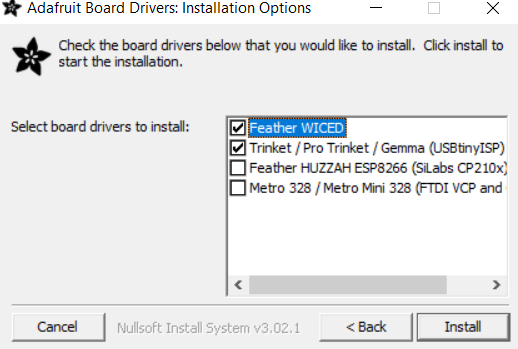
\includegraphics{/Users/davidlapuma/github/ctt_documentation/images/tinyUSB.png}

\begin{enumerate}
\def\labelenumi{\arabic{enumi}.}
\setcounter{enumi}{5}
\tightlist
\item
  Click \texttt{install}
\end{enumerate}

\hypertarget{im-using-usbasp-instead-of-usbtinyisp}{%
\subsubsection{\texorpdfstring{I'm using \texttt{USBasp} instead of
\texttt{USBtinyISP}}{I'm using USBasp instead of USBtinyISP}}\label{im-using-usbasp-instead-of-usbtinyisp}}

In order to run the above using the \texttt{USBasp} device instead of
the \texttt{USBtinyISP} programmer, please follow the steps below. Note
this \textbf{ONLY works on PC} computers so far\ldots so Mac users
should get the \texttt{USBtinyISP}.

\begin{enumerate}
\def\labelenumi{\arabic{enumi}.}
\tightlist
\item
  Install Arduino IDE 1.6.9 (scroll down on this page to find it:
  \url{https://www.arduino.cc/en/main/OldSoftwareReleases})
\end{enumerate}

\begin{itemize}
\tightlist
\item
  Note, if you have a previous version installed, this will uninstall
  that version before installing 1.6.9).
\end{itemize}

\begin{enumerate}
\def\labelenumi{\arabic{enumi}.}
\setcounter{enumi}{1}
\tightlist
\item
  Download and install \texttt{Zadig} (\url{https://zadig.akeo.ie})
\item
  Open \texttt{Zadig}
\item
  From the \texttt{Options} menu check the box for
  \texttt{List\ all\ devices}
\item
  Choose \texttt{USBAsp} from the dropdown list
\item
  select \texttt{libusb-win32\ (v1.2.6.0)} in the right menu
\end{enumerate}

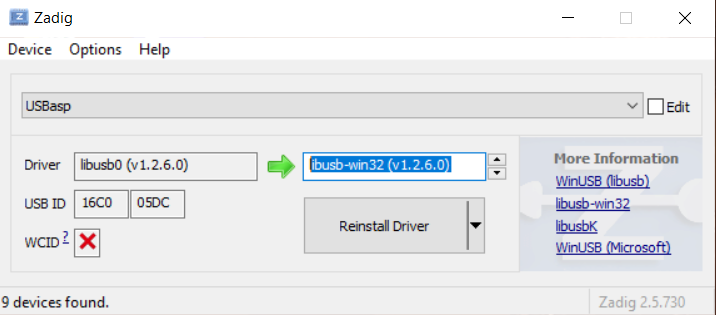
\includegraphics[width=0.5\textwidth,height=\textheight]{/Users/davidlapuma/github/ctt_documentation/images/zadig.png}

\begin{enumerate}
\def\labelenumi{\arabic{enumi}.}
\setcounter{enumi}{6}
\tightlist
\item
  select \texttt{reinstall\ driver}
\end{enumerate}

\end{document}
